
\documentclass[mathserif,serif]{beamer}
\usepackage[utf8]{inputenc}

\usepackage[T1]{fontenc}
\usepackage{graphicx}
\graphicspath{ {./images/} }
\usepackage{caption}
\captionsetup{font=scriptsize,labelfont=scriptsize}
\captionsetup[figure]{labelformat=empty}

\usetheme{Warsaw}
\usepackage{float}
\usepackage{pgf}  
\usepackage{multicol}
    
\titlegraphic
{
	\pgfputat{\pgfxy(0.7,-0.3)}{\pgfbox[center,base]{
\includegraphics[scale=0.3]{ufrgs}}}
}
\title{Estimativa da produção de energia de um parque eólico por meio de modelo estocástico}
\author{Diogo Friggo}
\institute{
	Universidade Federal do Rio Grande do Sul\newline\newline
	Orientador: Carlo Requião
	}
\date{Porto Alegre, 2018}
    
\begin{document}
    
%    \AtBeginSection[]
%    {
%      \begin{frame}
%        \frametitle{Sumário}
%        \tableofcontents[currentsection]
%      \end{frame}
%    }
%    
%    \AtBeginSubsection[]
%    {
%      \begin{frame}
%        \frametitle{Sumário}
%        \tableofcontents[currentsection,currentsubsection]
%      \end{frame}
%    }

%{ 
%\usebackgroundtemplate{\includegraphics[width=\paperwidth,height=\paperheight]{osorio}} 

\frame{\titlepage}

\frame {
        \frametitle{Energia eólica}
        
		O investimento em energia eólica vem crescendo em todo o mundo:\newline
        
        \begin{itemize}
        \item Alternativa a fontes de energia não-renováveis
        \item Capaz de suprir boa parte da demanda de um país
        \item Economicamente viável
        \item Décadas de experiência acumulada
        \end{itemize}
    }

\frame{\frametitle{Energia eólica: em crescimento}\begin{figure}[h]
    \centering
	\includegraphics[scale=0.47]{19802010}
	\caption{Geração de energia. Fonte: EPE.}
\end{figure}}

\frame{\frametitle{O recurso eólico nacional}\begin{figure}[h]
    \centering
	\includegraphics[scale=0.5]{brasilpotencialeolico}
	\caption{O potencial eólico do Brasil. Fonte: CEPEL.}
\end{figure}}

\frame{\frametitle{O cálculo da potência}

\begin{equation*}
	P = \frac{1}{2}\rho \frac{\pi D^2}{4}\nu^3C_p\eta
\end{equation*}

\begin{flalign*}
P &= \mbox{potência elétrica na altura do cubo rotor}\left[W\right]&&\\
\rho &= \mbox{densidade do ar}\left[\frac{kg}{m^3}\right]&&\\
D &= \mbox{diâmetro do rotor}\left[m\right]&&\\\nonumber
\nu &= \mbox{velocidade do vento} \left[\frac{m}{s}\right]&&\\\nonumber
C_p &= \mbox{coeficiente aerodinâmico de potência do rotor}\left[W\right]&&\\\nonumber
\eta &= \mbox{eficiência do conjunto gerador/transmissão}&&\\\nonumber
\end{flalign*}

}

\frame{\frametitle{Consumo médio residencial}\begin{figure}[h]
    \centering
	\includegraphics[width=\textwidth]{consumoresidencial}
	\caption{Consumo médio residencial no país. Fonte: EPE.}
\end{figure}}

\frame{\frametitle{Dados de vento ERA 5: cidade de Sento Sé}\begin{figure}[h]
    \centering
	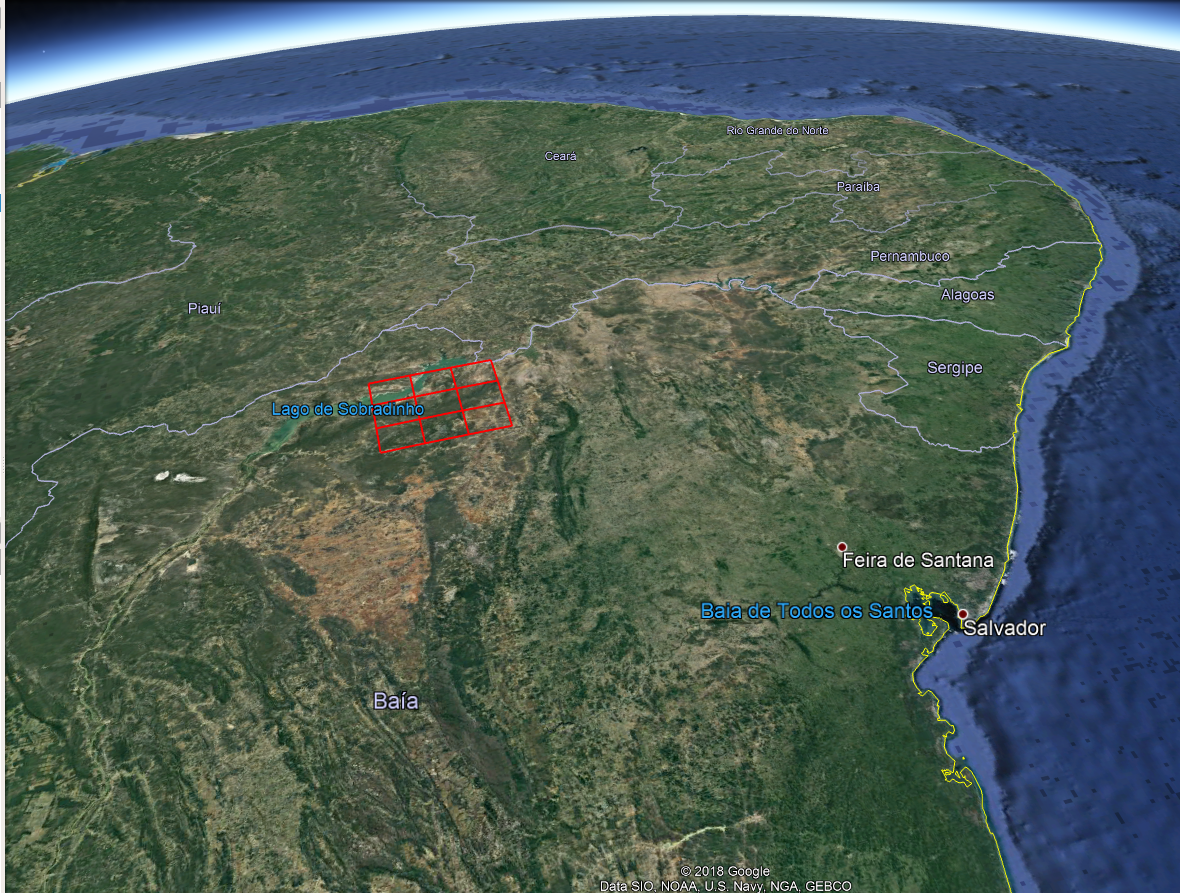
\includegraphics[scale=0.6]{earth}
	\caption{Localização da região de medição por satélite da cidade de Sento Sé. Fonte: SIO, NOAA, U.S. Navy, NGA, GEBCO. \textcopyright \  2018 Google}
\end{figure}}

\frame{\frametitle{Rosa dos ventos anual}\begin{figure}[h]
    \centering
	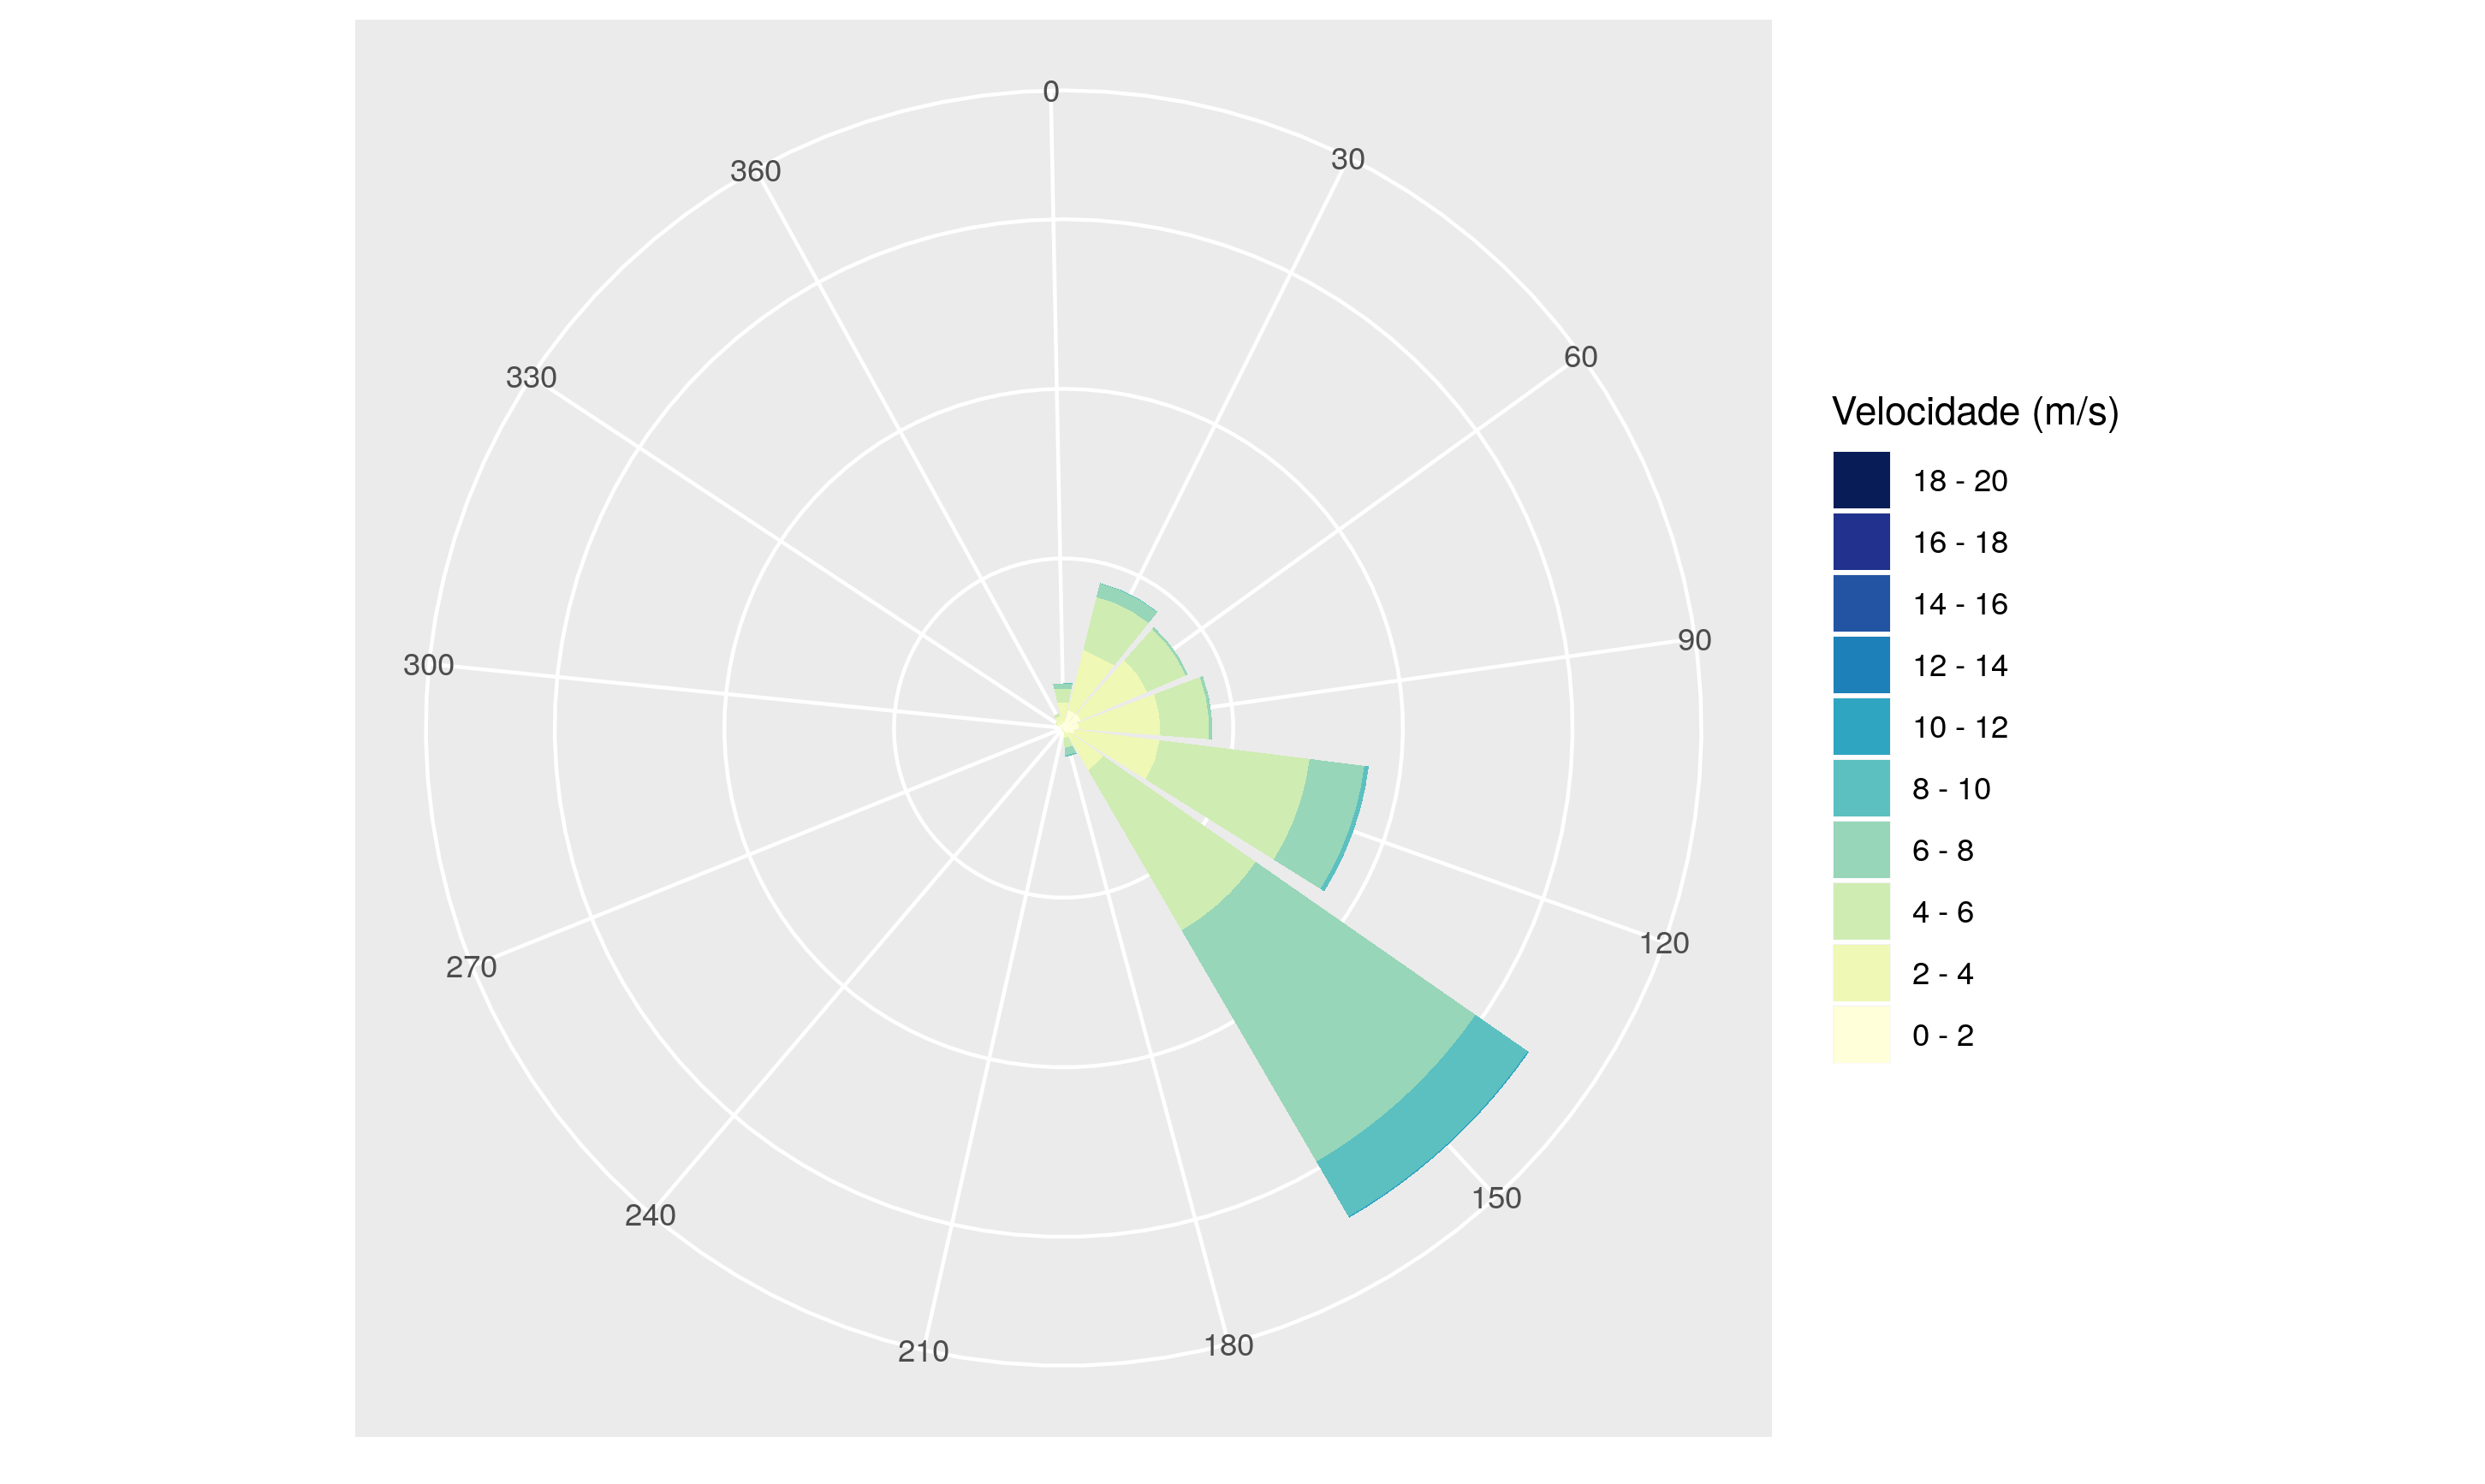
\includegraphics[scale=0.55]{windrose}
	\caption{Rosa dos ventos do recurso eólico da cidade de Sento Sé no norte da Bahia. Fonte: autoria própria, dados: ECWMF.}
\end{figure}}

\frame{\frametitle{Rosas dos ventos mensais}\begin{figure}[h]
    \centering
%  	\hspace*{-1.4cm}   
	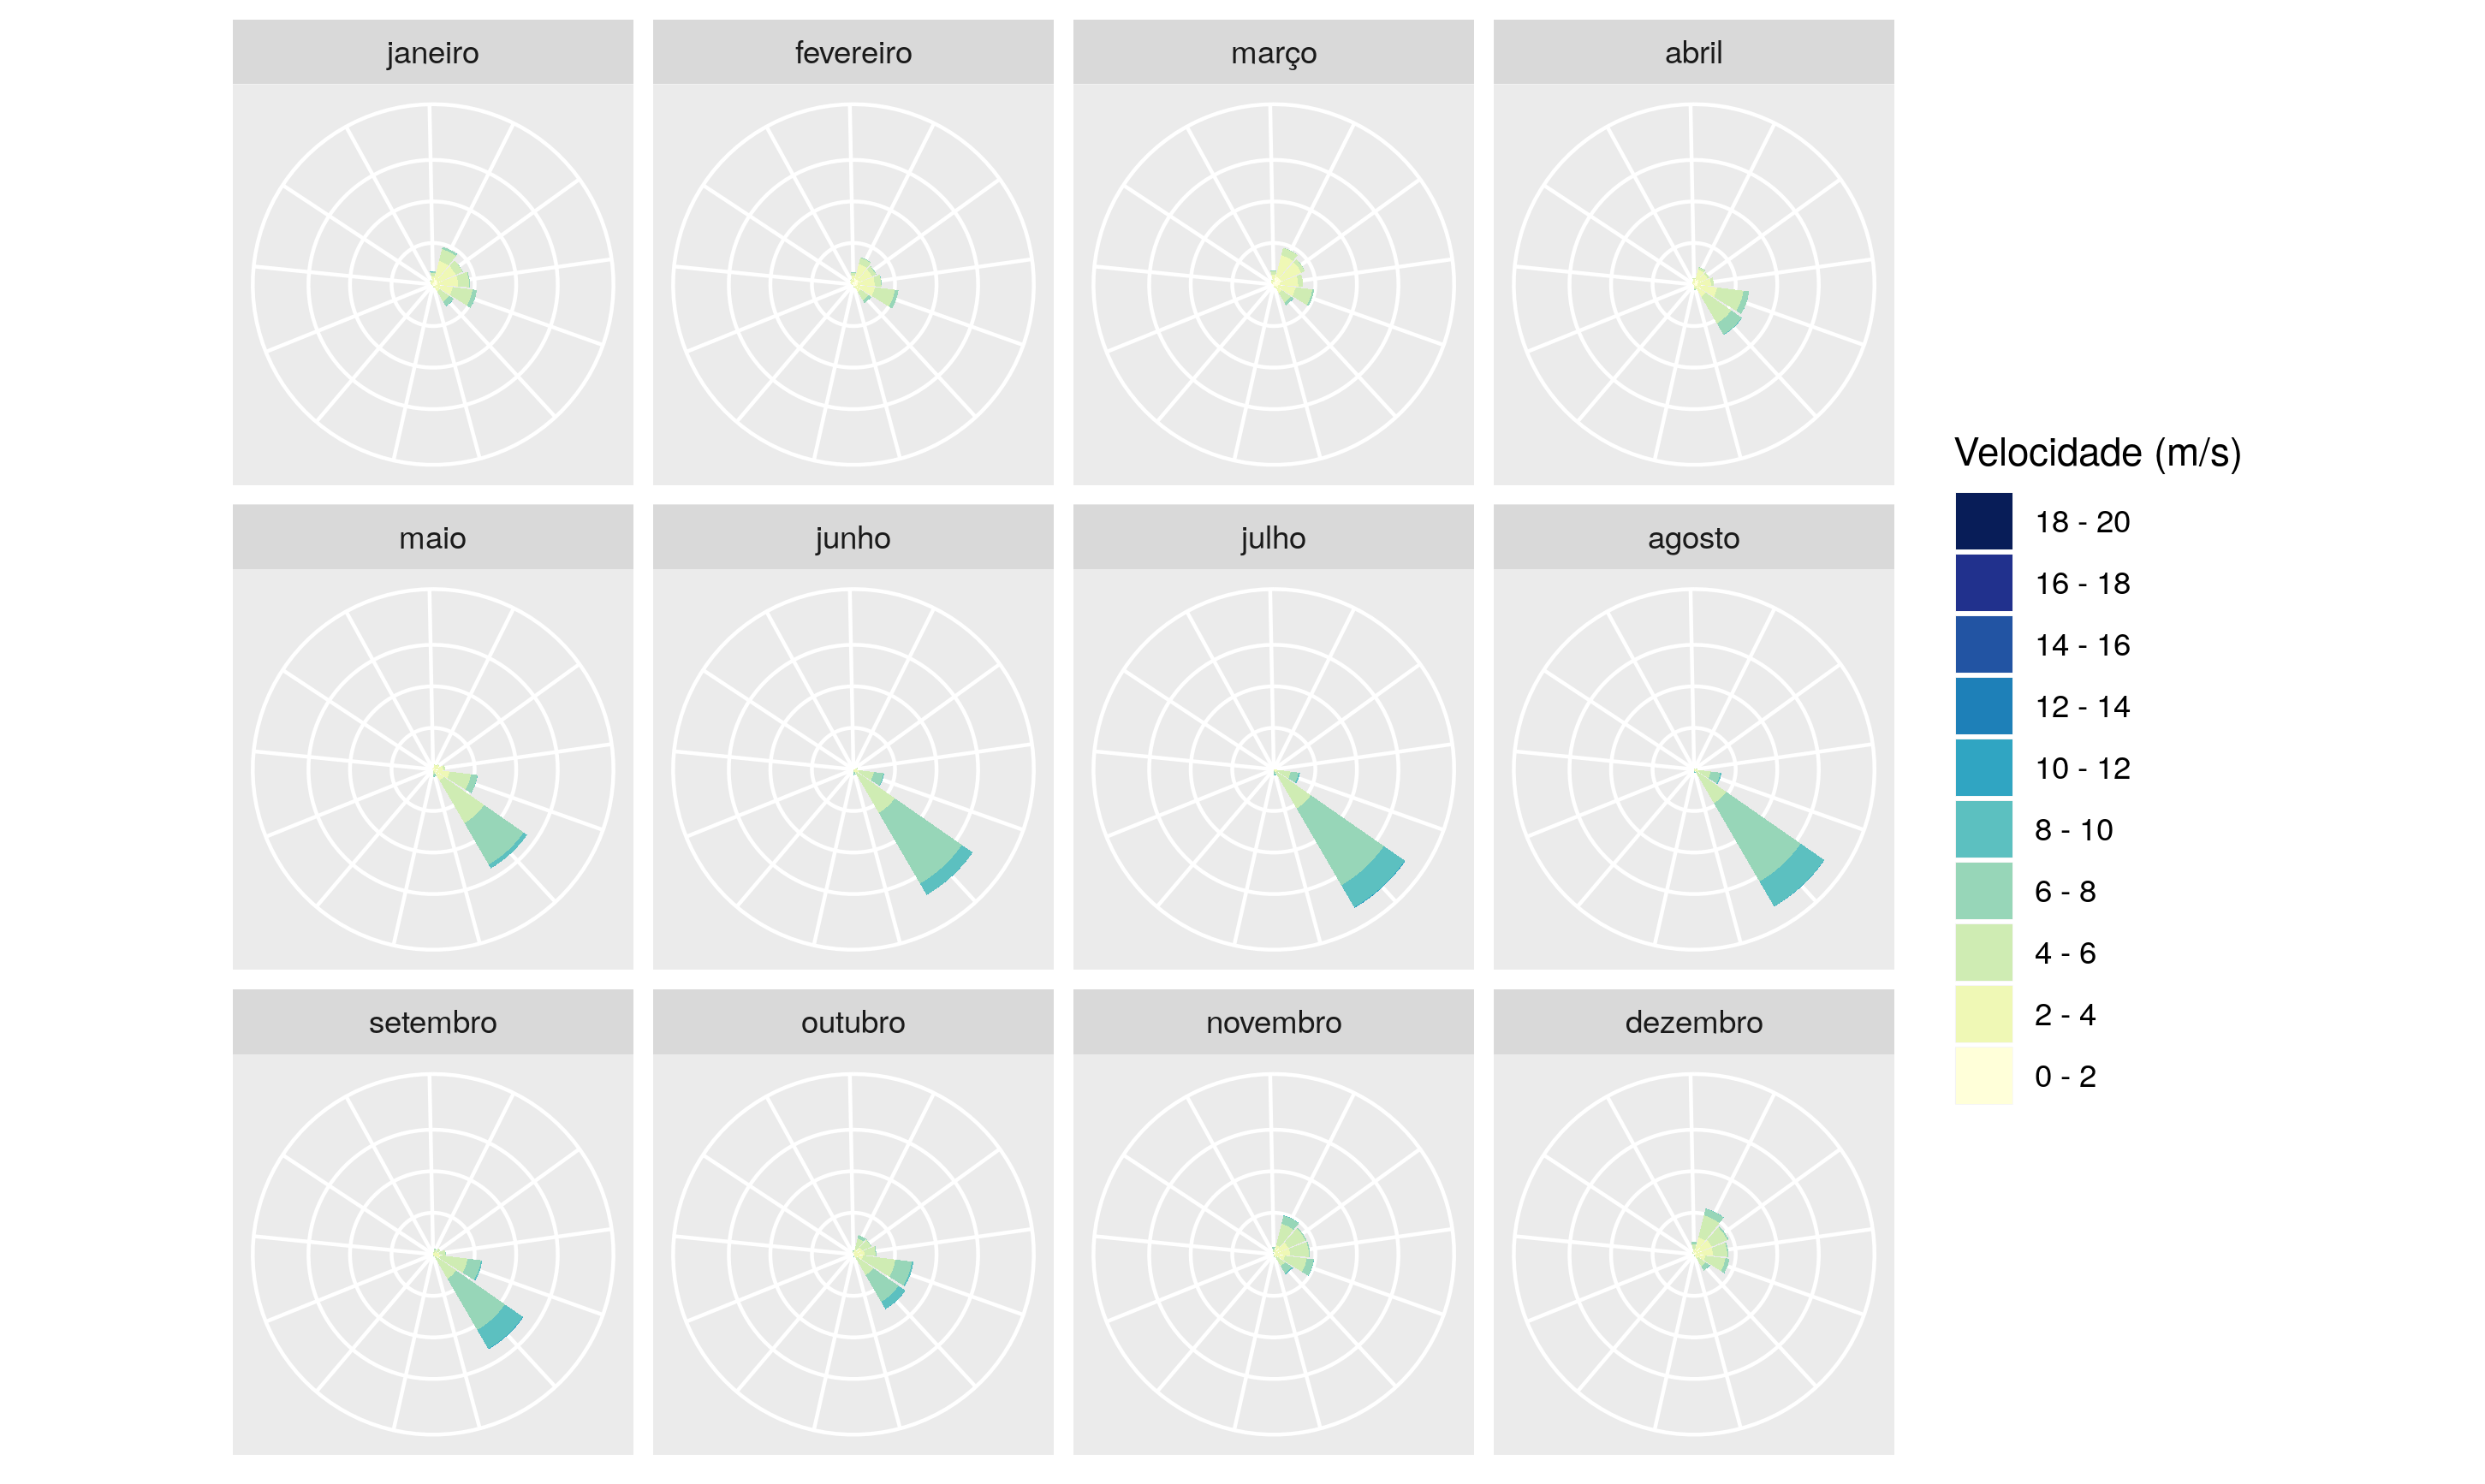
\includegraphics[scale=0.55]{windrose_monthly}
	\caption{Rosas dos ventos mensais do recurso eólico da cidade de Sento Sé. Fonte: autoria própria, dados: ECWMF.}
\end{figure}}

\frame{\frametitle{O Jogo do Caos}
	Regras
	\begin{itemize}
		\item Desenhe 3 pontos (x1,x2, x3). Identifique esses pontos com os número de um dado: 1 (1,4), 2 (2,5), 3 (3,6)
		\item Desenhe um outro ponto qualquer (x0).
		\item Jogue um dado. Se o número for 2 ou 5, por exemplo, marque outro ponto no meio da linha que liga x0 a x2
		\item Jogue o dado novamente e faça o mesmo considerando o ponto x0 como o ponto desenhado anteriormente
	\end{itemize}
}
\begin{frame}
\frametitle{O Jogo do Caos}
\begin{columns}[t]
\column{.5\textwidth}
\centering
\fbox{\includegraphics[scale=0.5]{first}}\\
\vspace{0.5cm}
\fbox{\includegraphics[scale=0.5]{third}}\\
\column{.5\textwidth}
\centering
\vspace{0.5cm}
\fbox{\includegraphics[scale=0.5]{second}}
\fbox{\includegraphics[scale=0.5]{last}}
\end{columns}

\vspace{0.5cm}
O Jogo do Caos. Fonte: Wikimedia Commons. CC BY-SA 3.0
\end{frame}

\frame{\frametitle{Triângulo de Sierpinski}\begin{figure}[h]
    \centering
	\includegraphics[scale=0.2]{triangle}
	\caption{Triângulo de Sierpinski. Fonte: Wikimedia Commons. CC BY-SA 3.0}
\end{figure}}

\frame{\frametitle{O caráter estocástico do vento: anual}\begin{figure}[h]
    \centering
	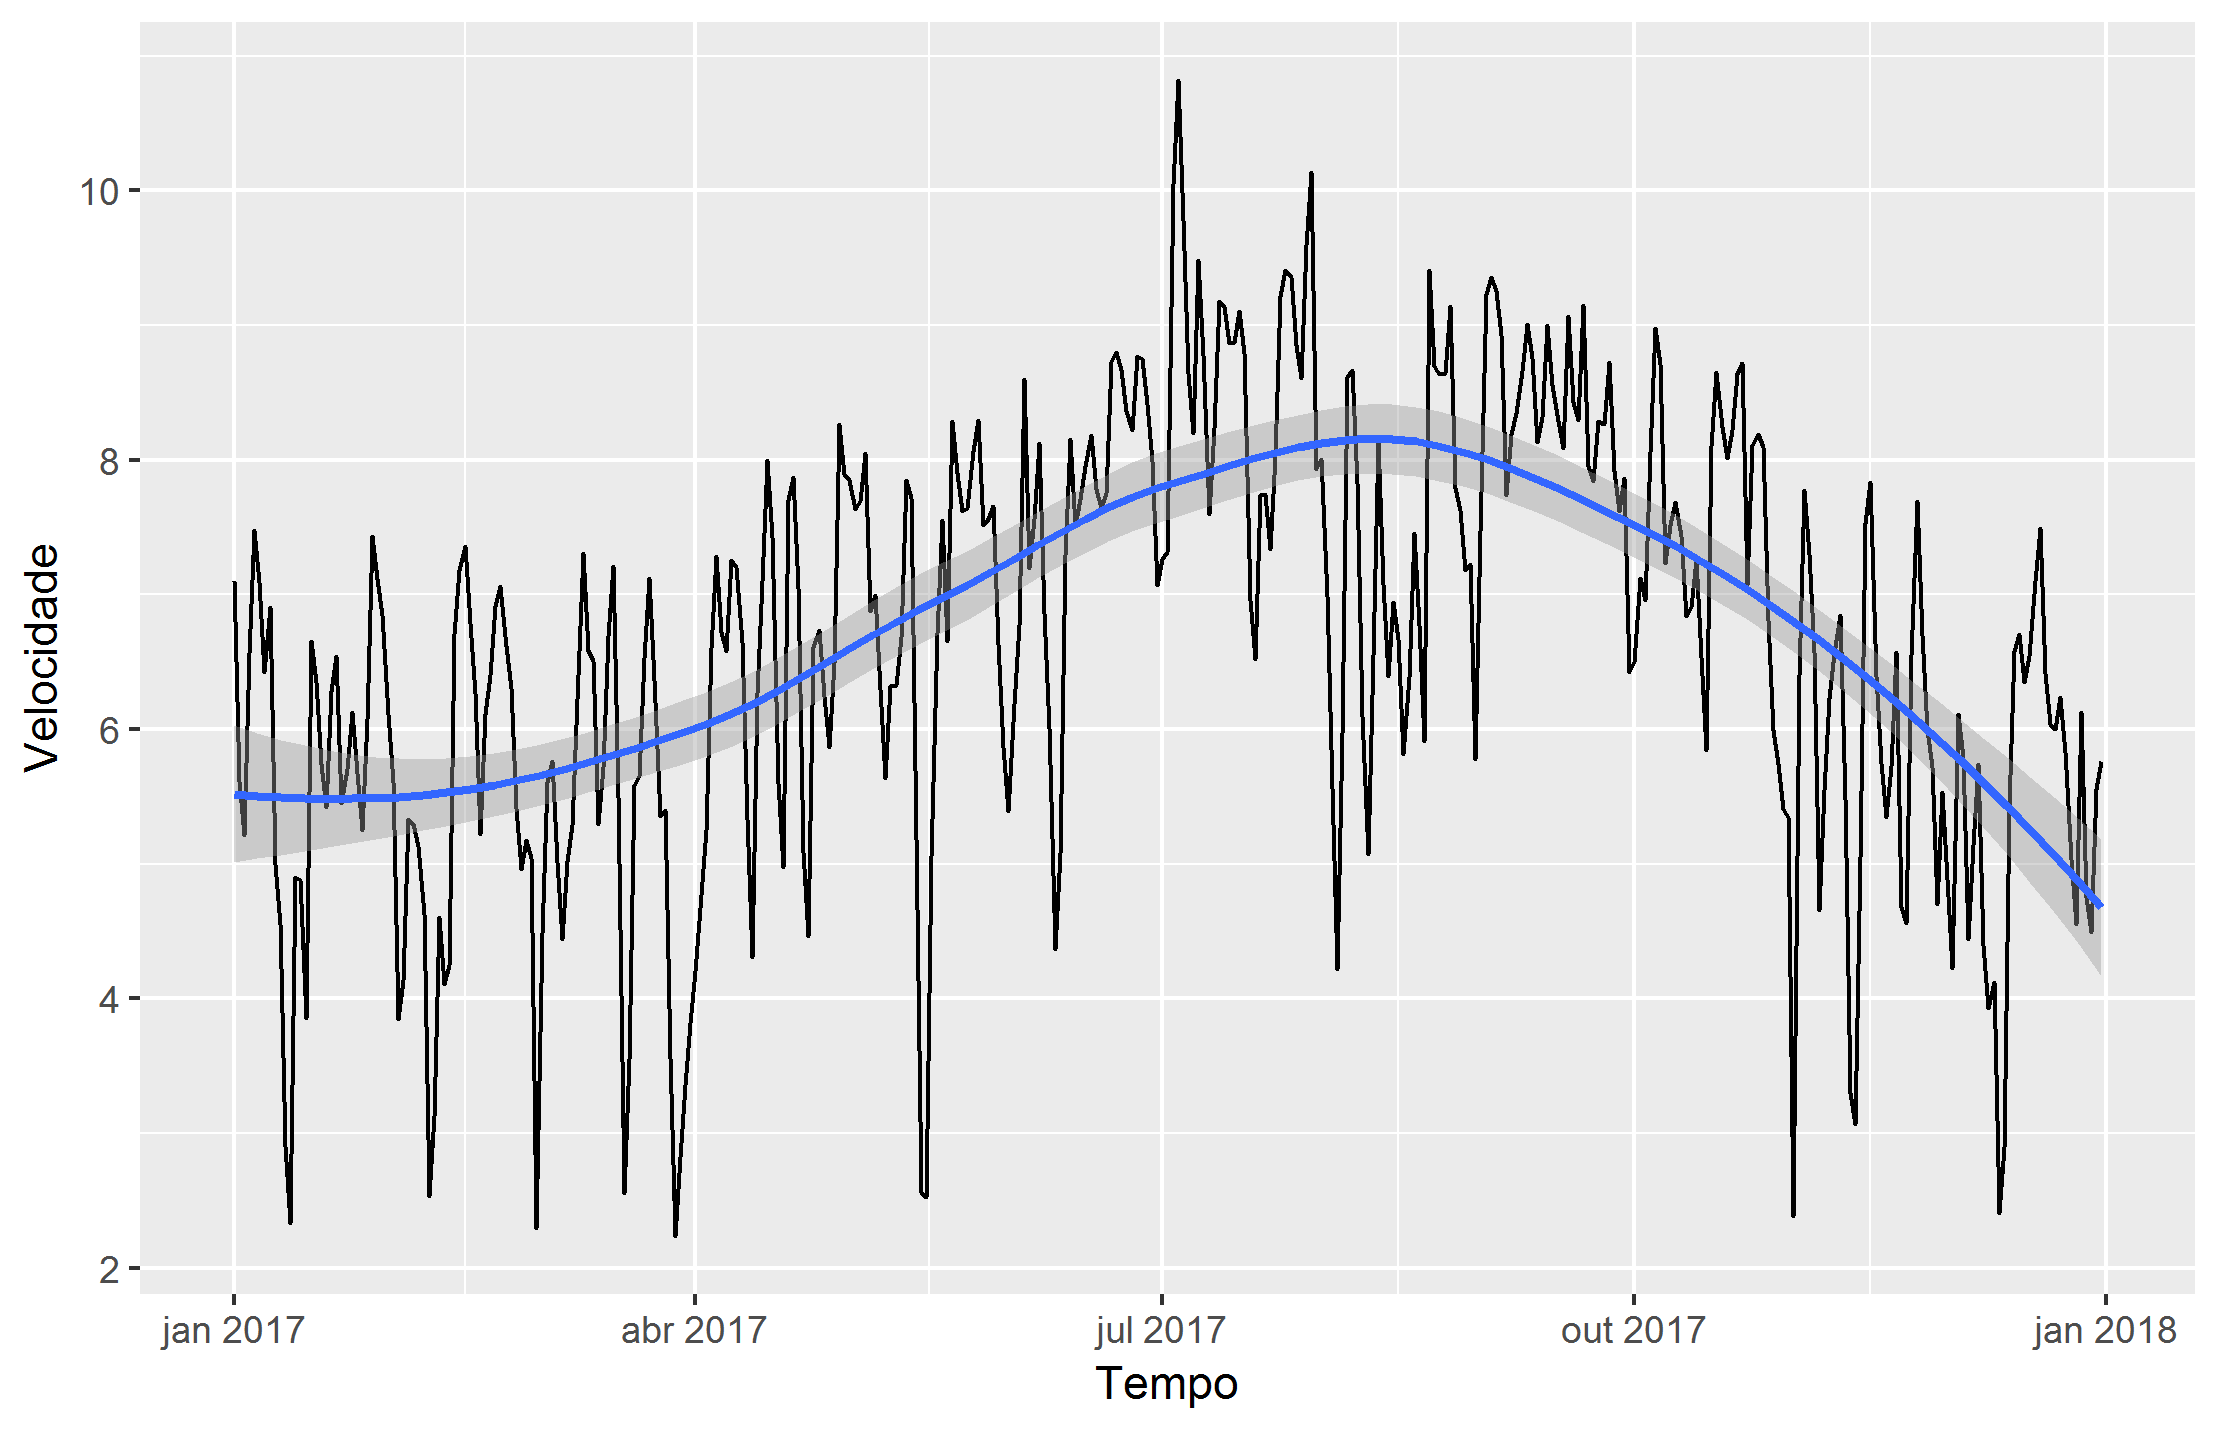
\includegraphics[scale=0.55]{stochastic}
	\caption{Velocidade do vento medida por satélite na cidade de Sento Sé. Fonte: autoria própria. Dados: ECWMF. Curva em azul: ajuste aos dados medidos, dados: ECMWF}
\end{figure}}

\frame{\frametitle{O caráter estocástico do vento: mensal}\begin{figure}[h]
    \centering
	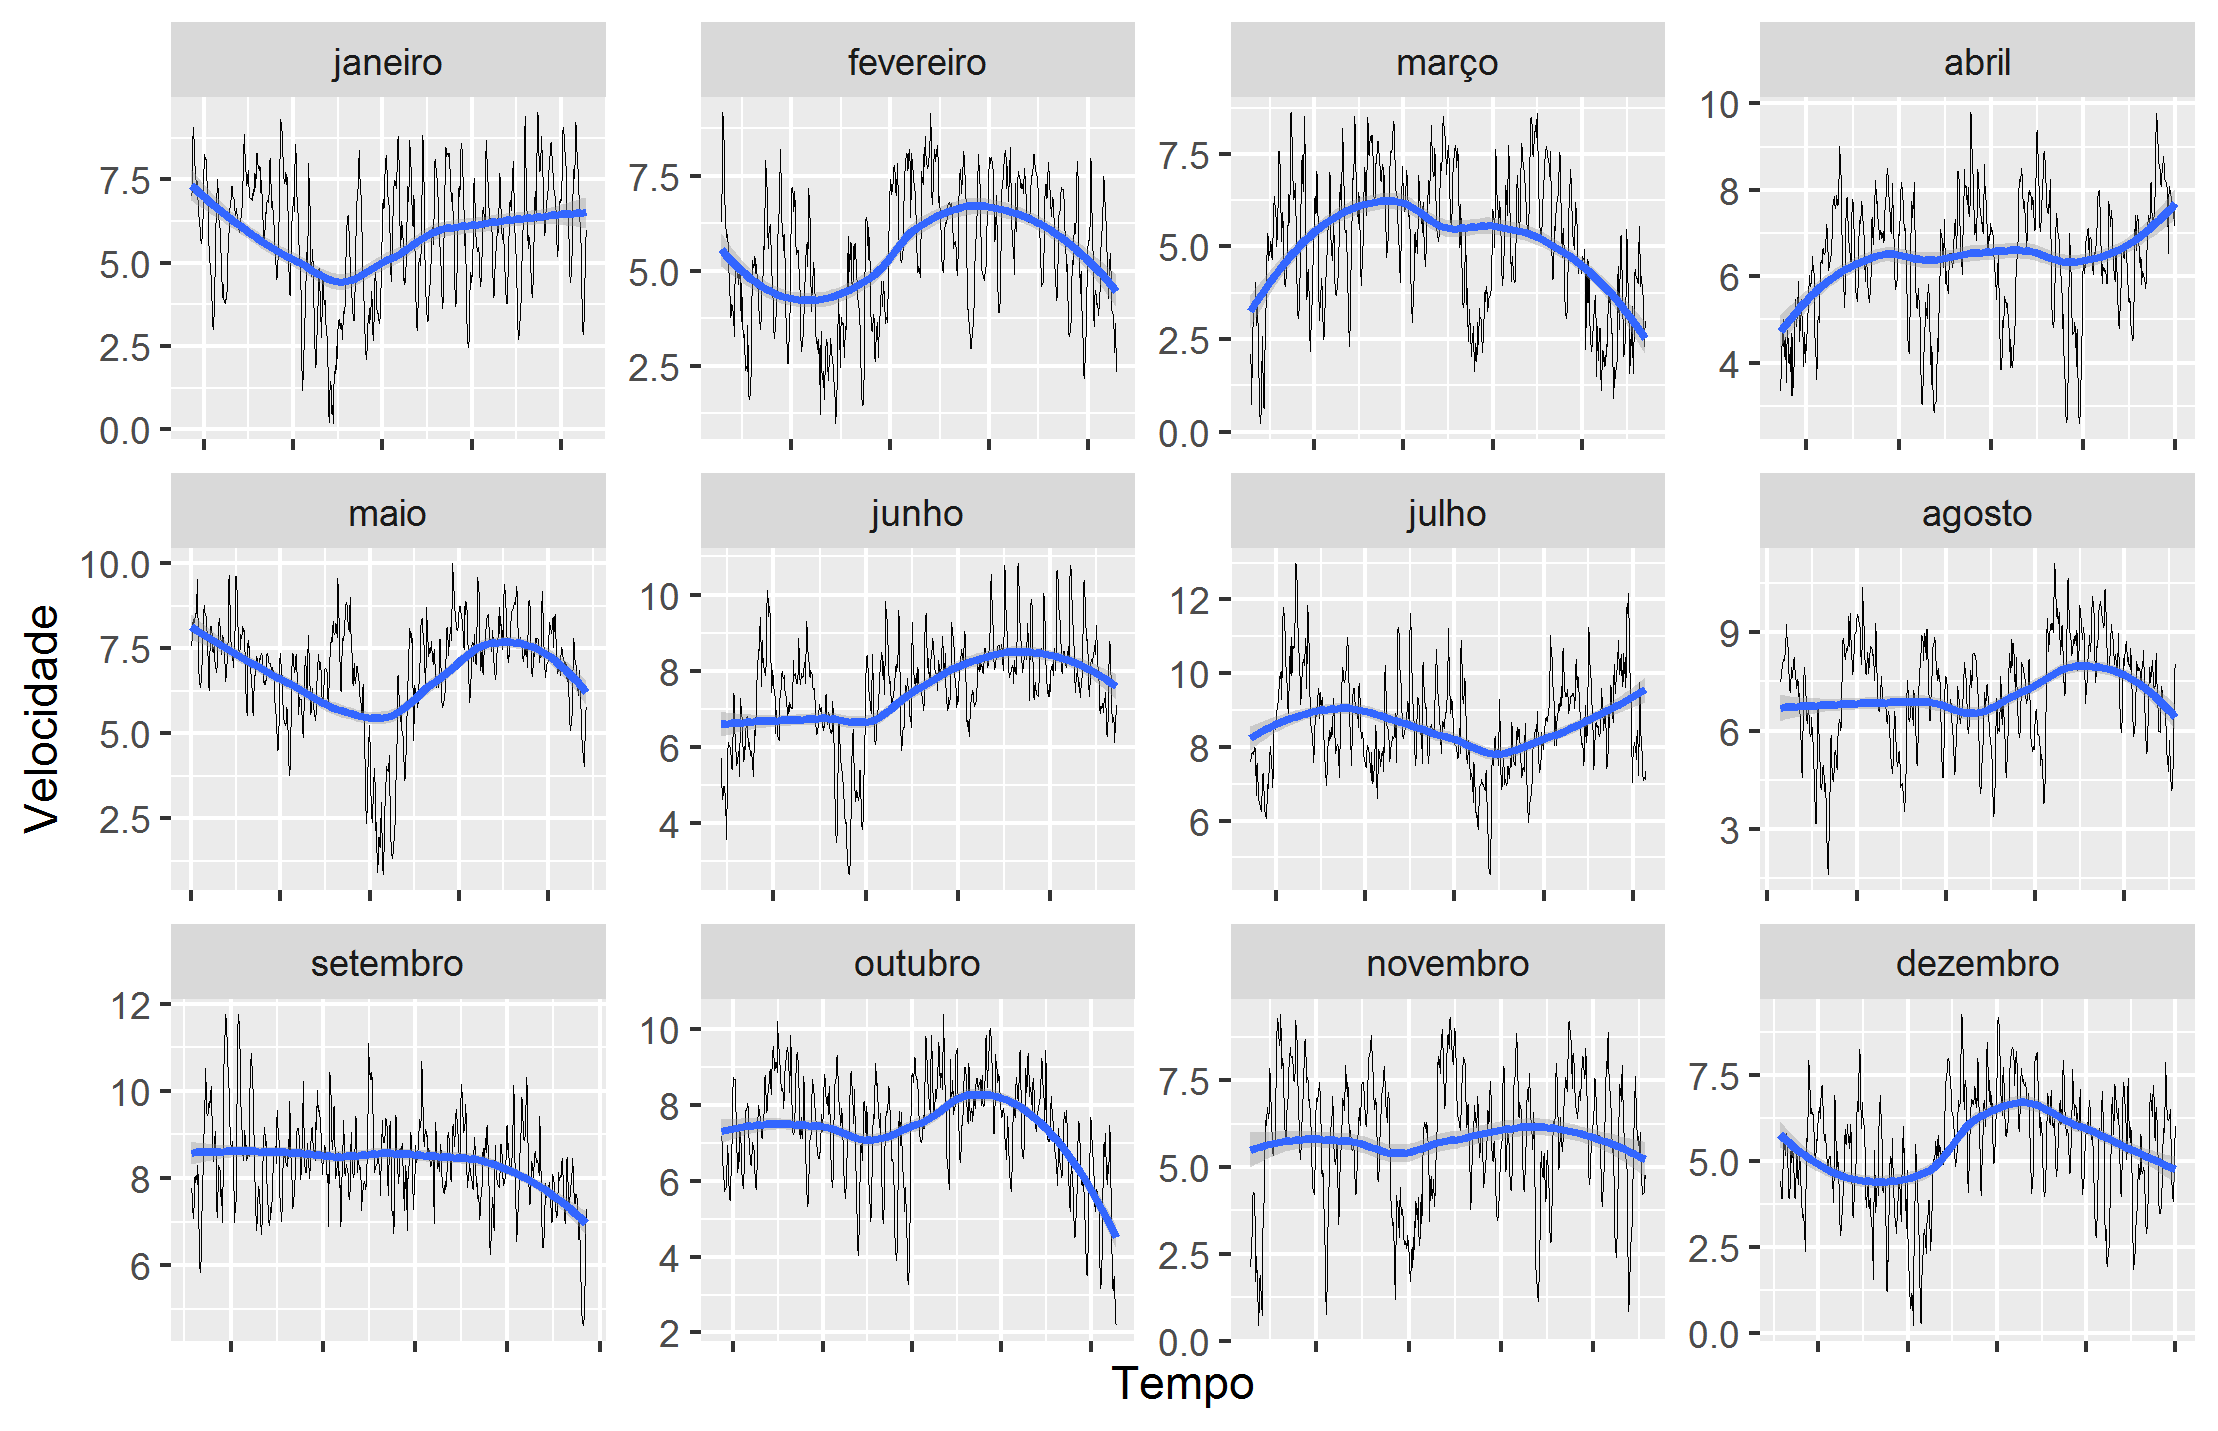
\includegraphics[scale=0.53]{stochastic_monthly}
	\caption{Velocidade do vento para cada mês do ano de 2017 da cidade de Sento Sé no norte da Bahia. Curva em preto: dados medidos. Curva em azul: ajuste aos dados medidos. Fonte: autoria própria, dados: ECMWF.}
\end{figure}}

\frame{\frametitle{Ordem em meio ao caos}\begin{figure}[h]
    \centering
	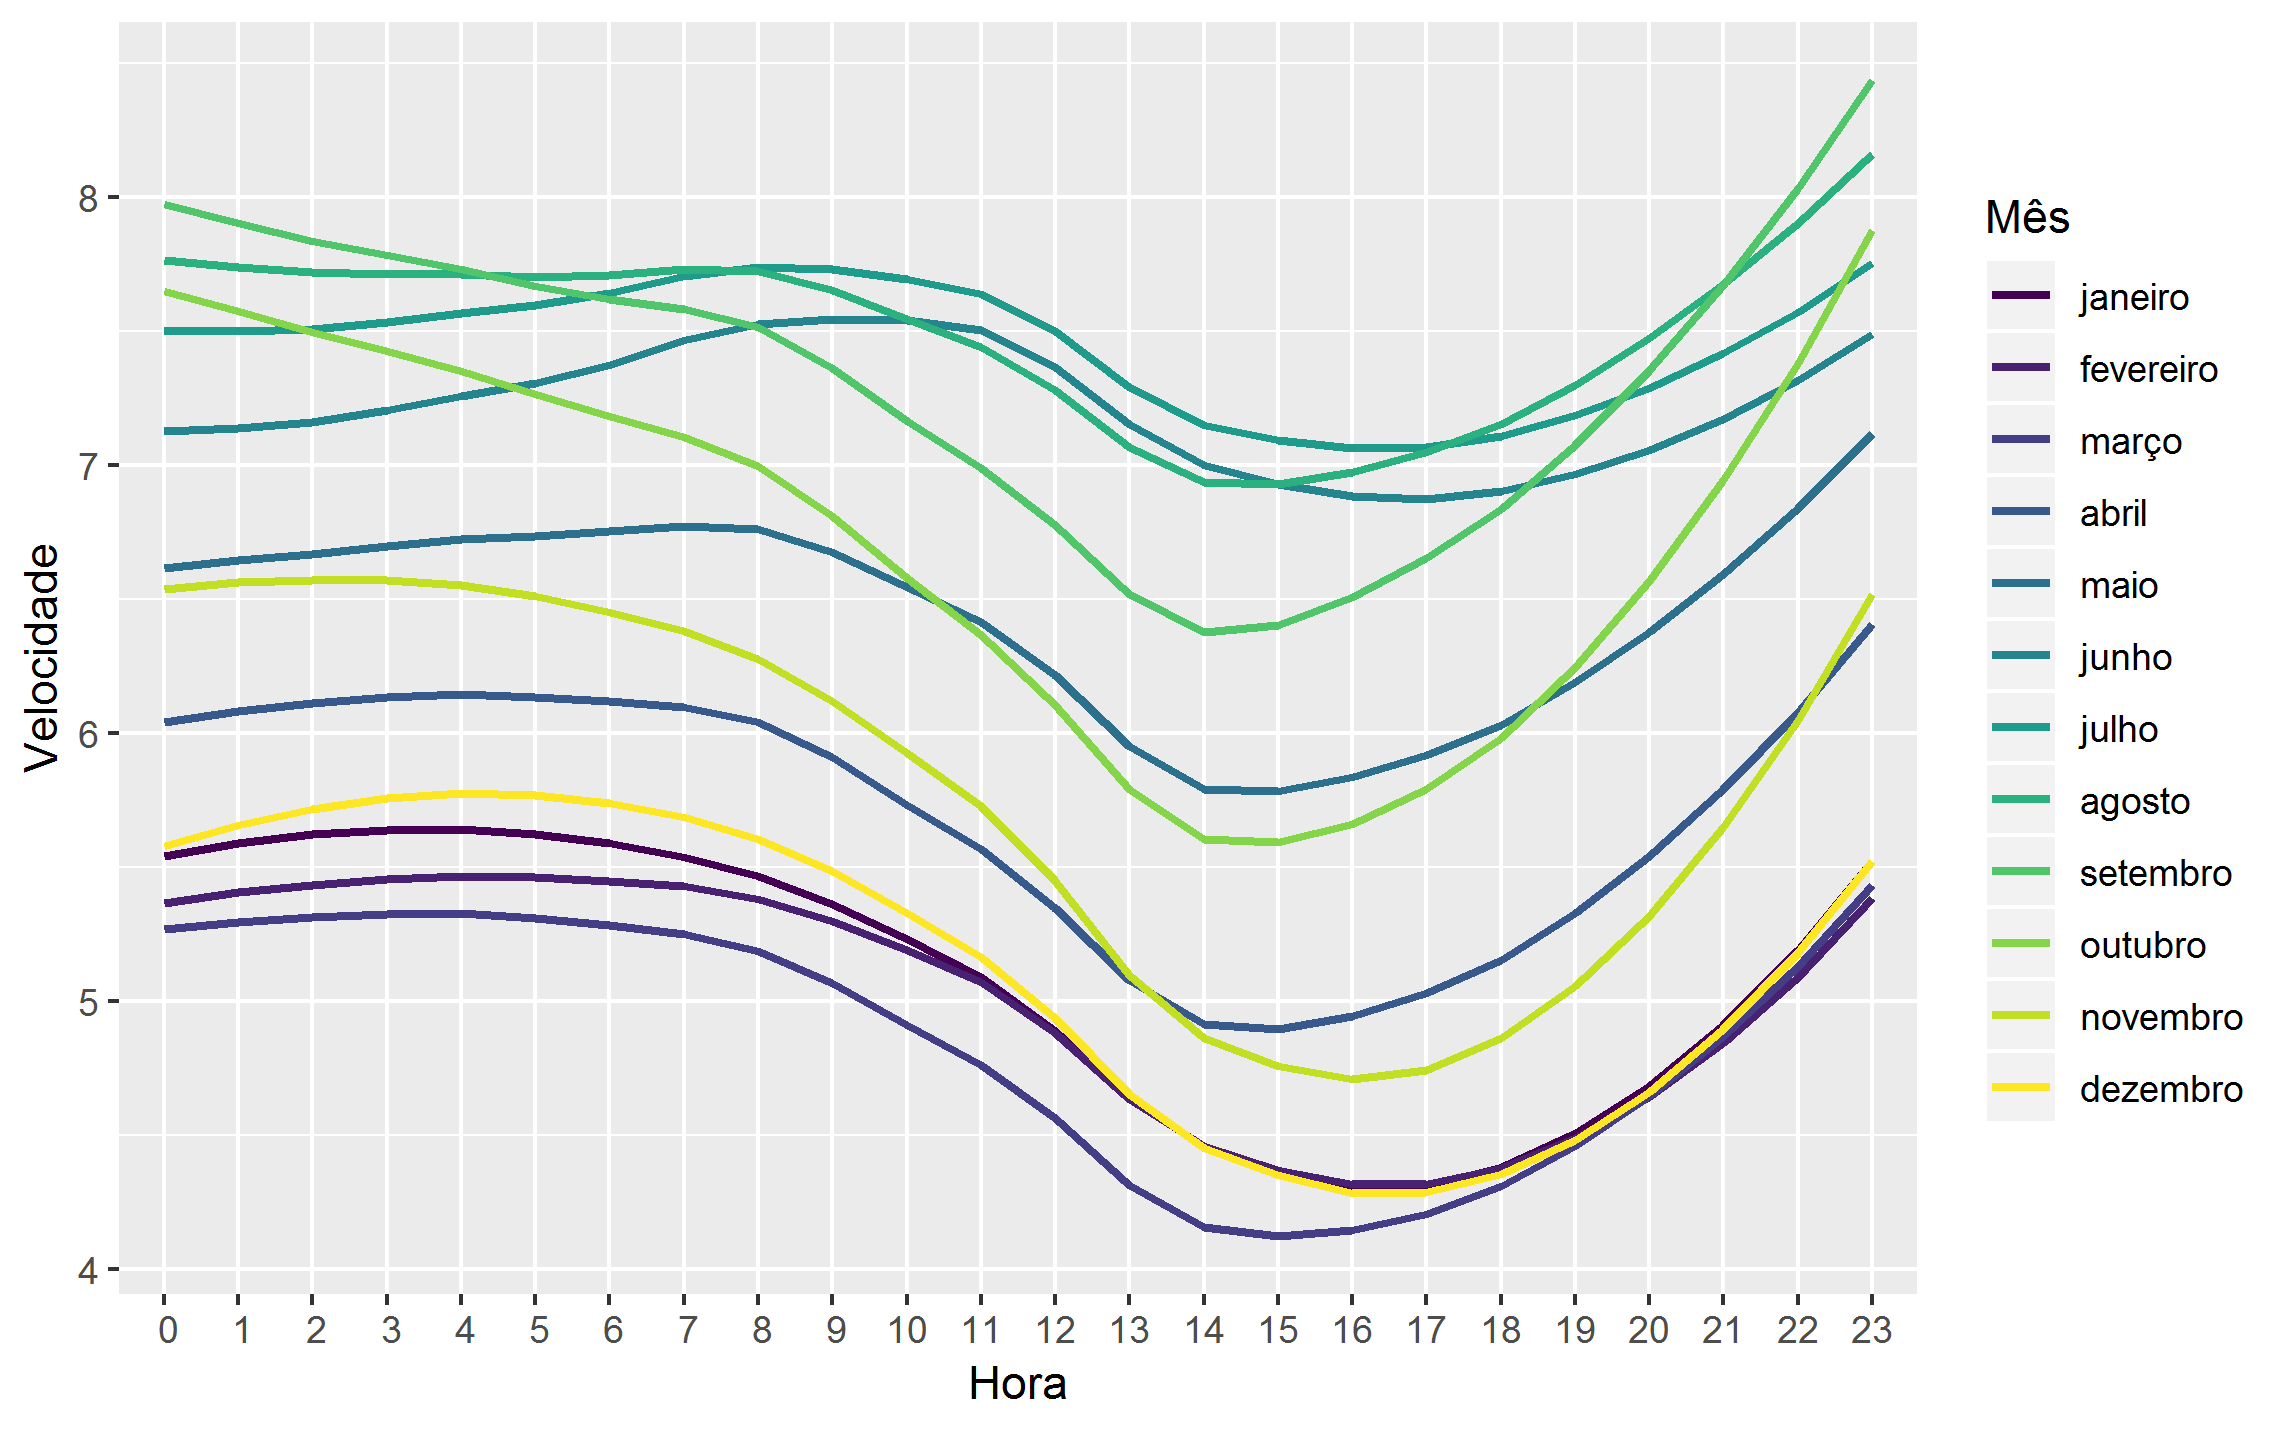
\includegraphics[width=\textwidth]{diurnal}
	\caption{Velocidade do vento para cada hora do dia e para cada mês do ano de 2017. Fonte: autoria própria, dados: ECWMF.}
\end{figure}}

\frame{\frametitle{Precisão numérica}\begin{figure}[h]
    \centering
	\includegraphics[scale=0.8]{grid}
	\caption{Grid de medições. Fonte: Earth Magazine.}
\end{figure}}

\frame{\frametitle{Recurso eólico de longo prazo: distribuição de Weibull}\begin{figure}[h]
    \centering
	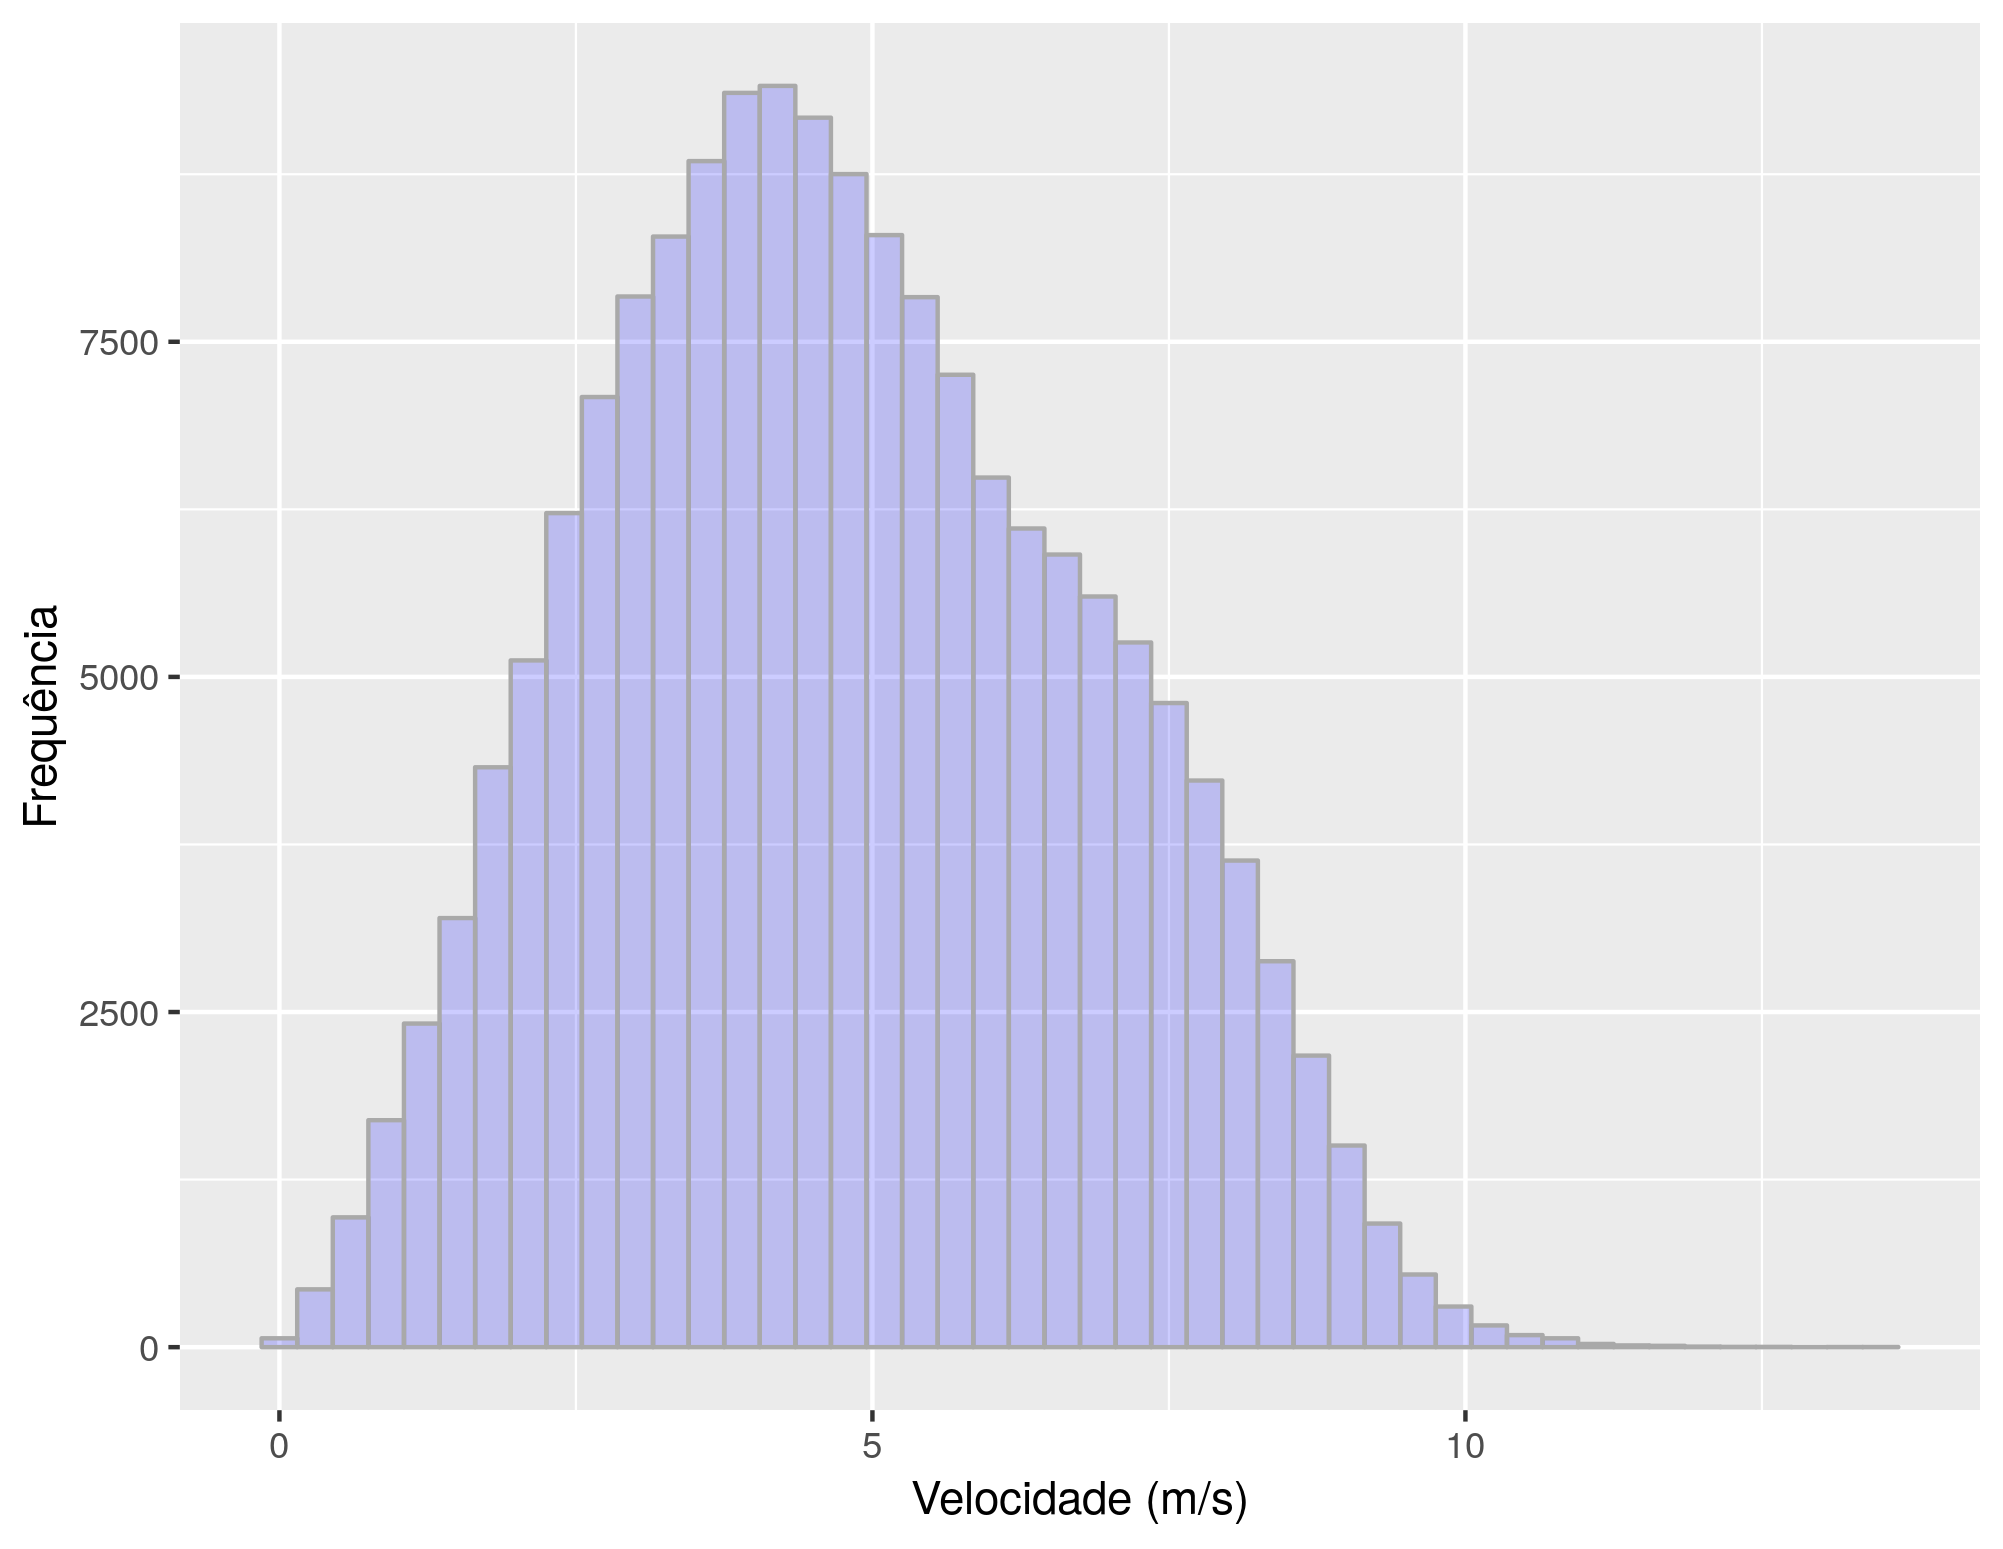
\includegraphics[scale=0.55]{weibull_histogram}
	\caption{A distribuição de velocidades do quadrante central. Fonte: autoria própria, dados: ECWMF.}
\end{figure}}

\frame{\frametitle{Recurso eólico de longo prazo: distribuição de Weibull}\begin{figure}[h]
    \centering
	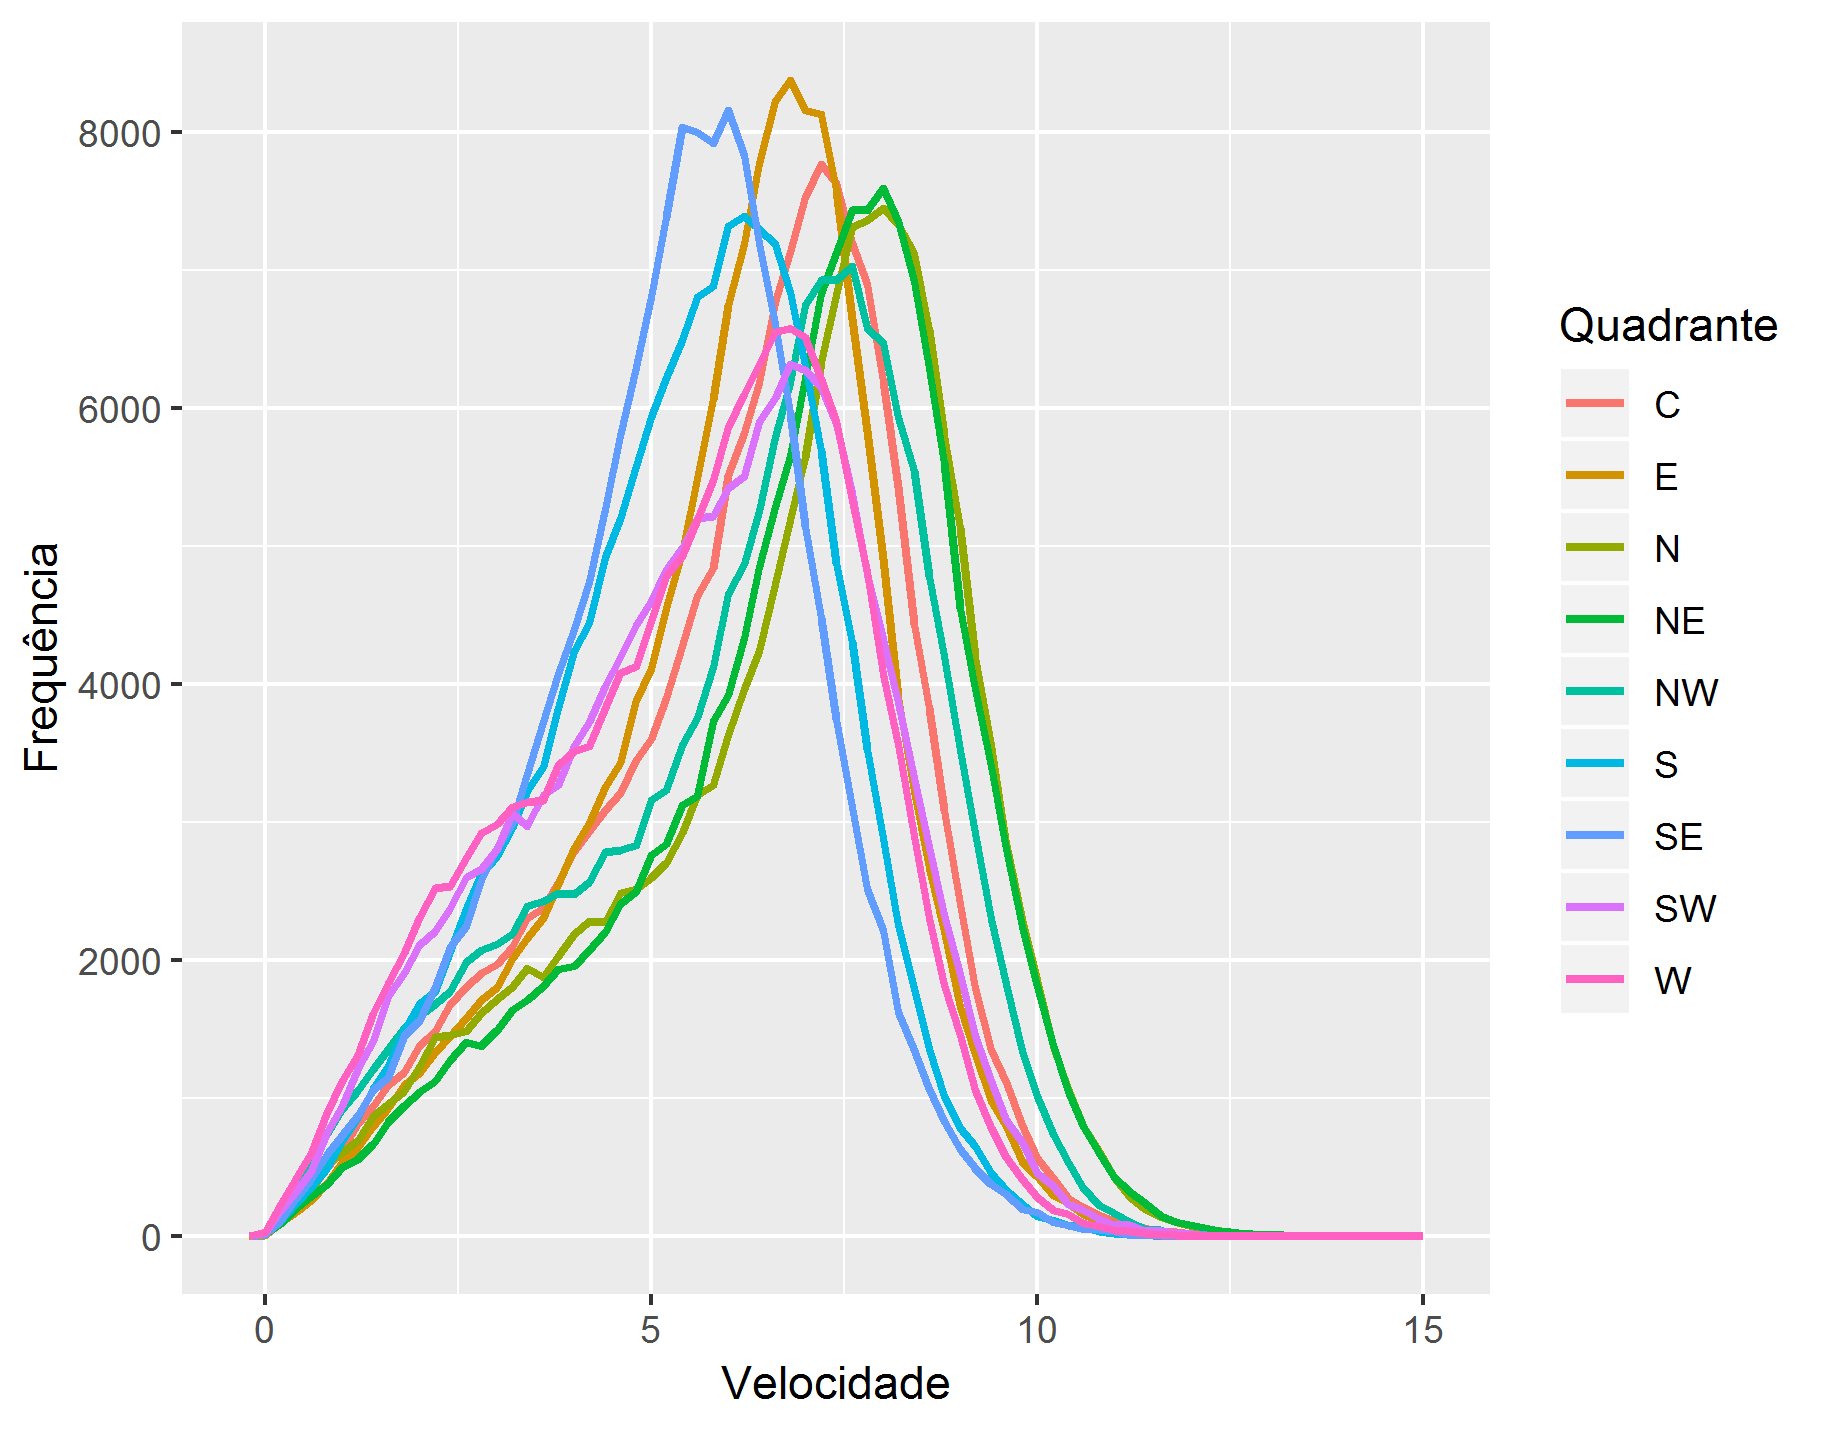
\includegraphics[scale=0.55]{weibull_freqpoly}
	\caption{Distribuição de velocidades de todos os quadrantes. Fonte: autoria própria, dados: ECWMF.}
\end{figure}}

    \frame
    {
        \frametitle{Resolução temporal}
Estimativa do recurso eólico em base mensal, diária, horária?
\begin{itemize}
\item 	mensal: negociação mais sólida com investidores
\item 	diária: minimizar perdas por manutenção
\item 	horária: adequamento da oferta de energia ao consumo local
\end{itemize}
    }

\frame{\frametitle{O cálculo estocástico na economia}\begin{figure}[h]
    \centering
	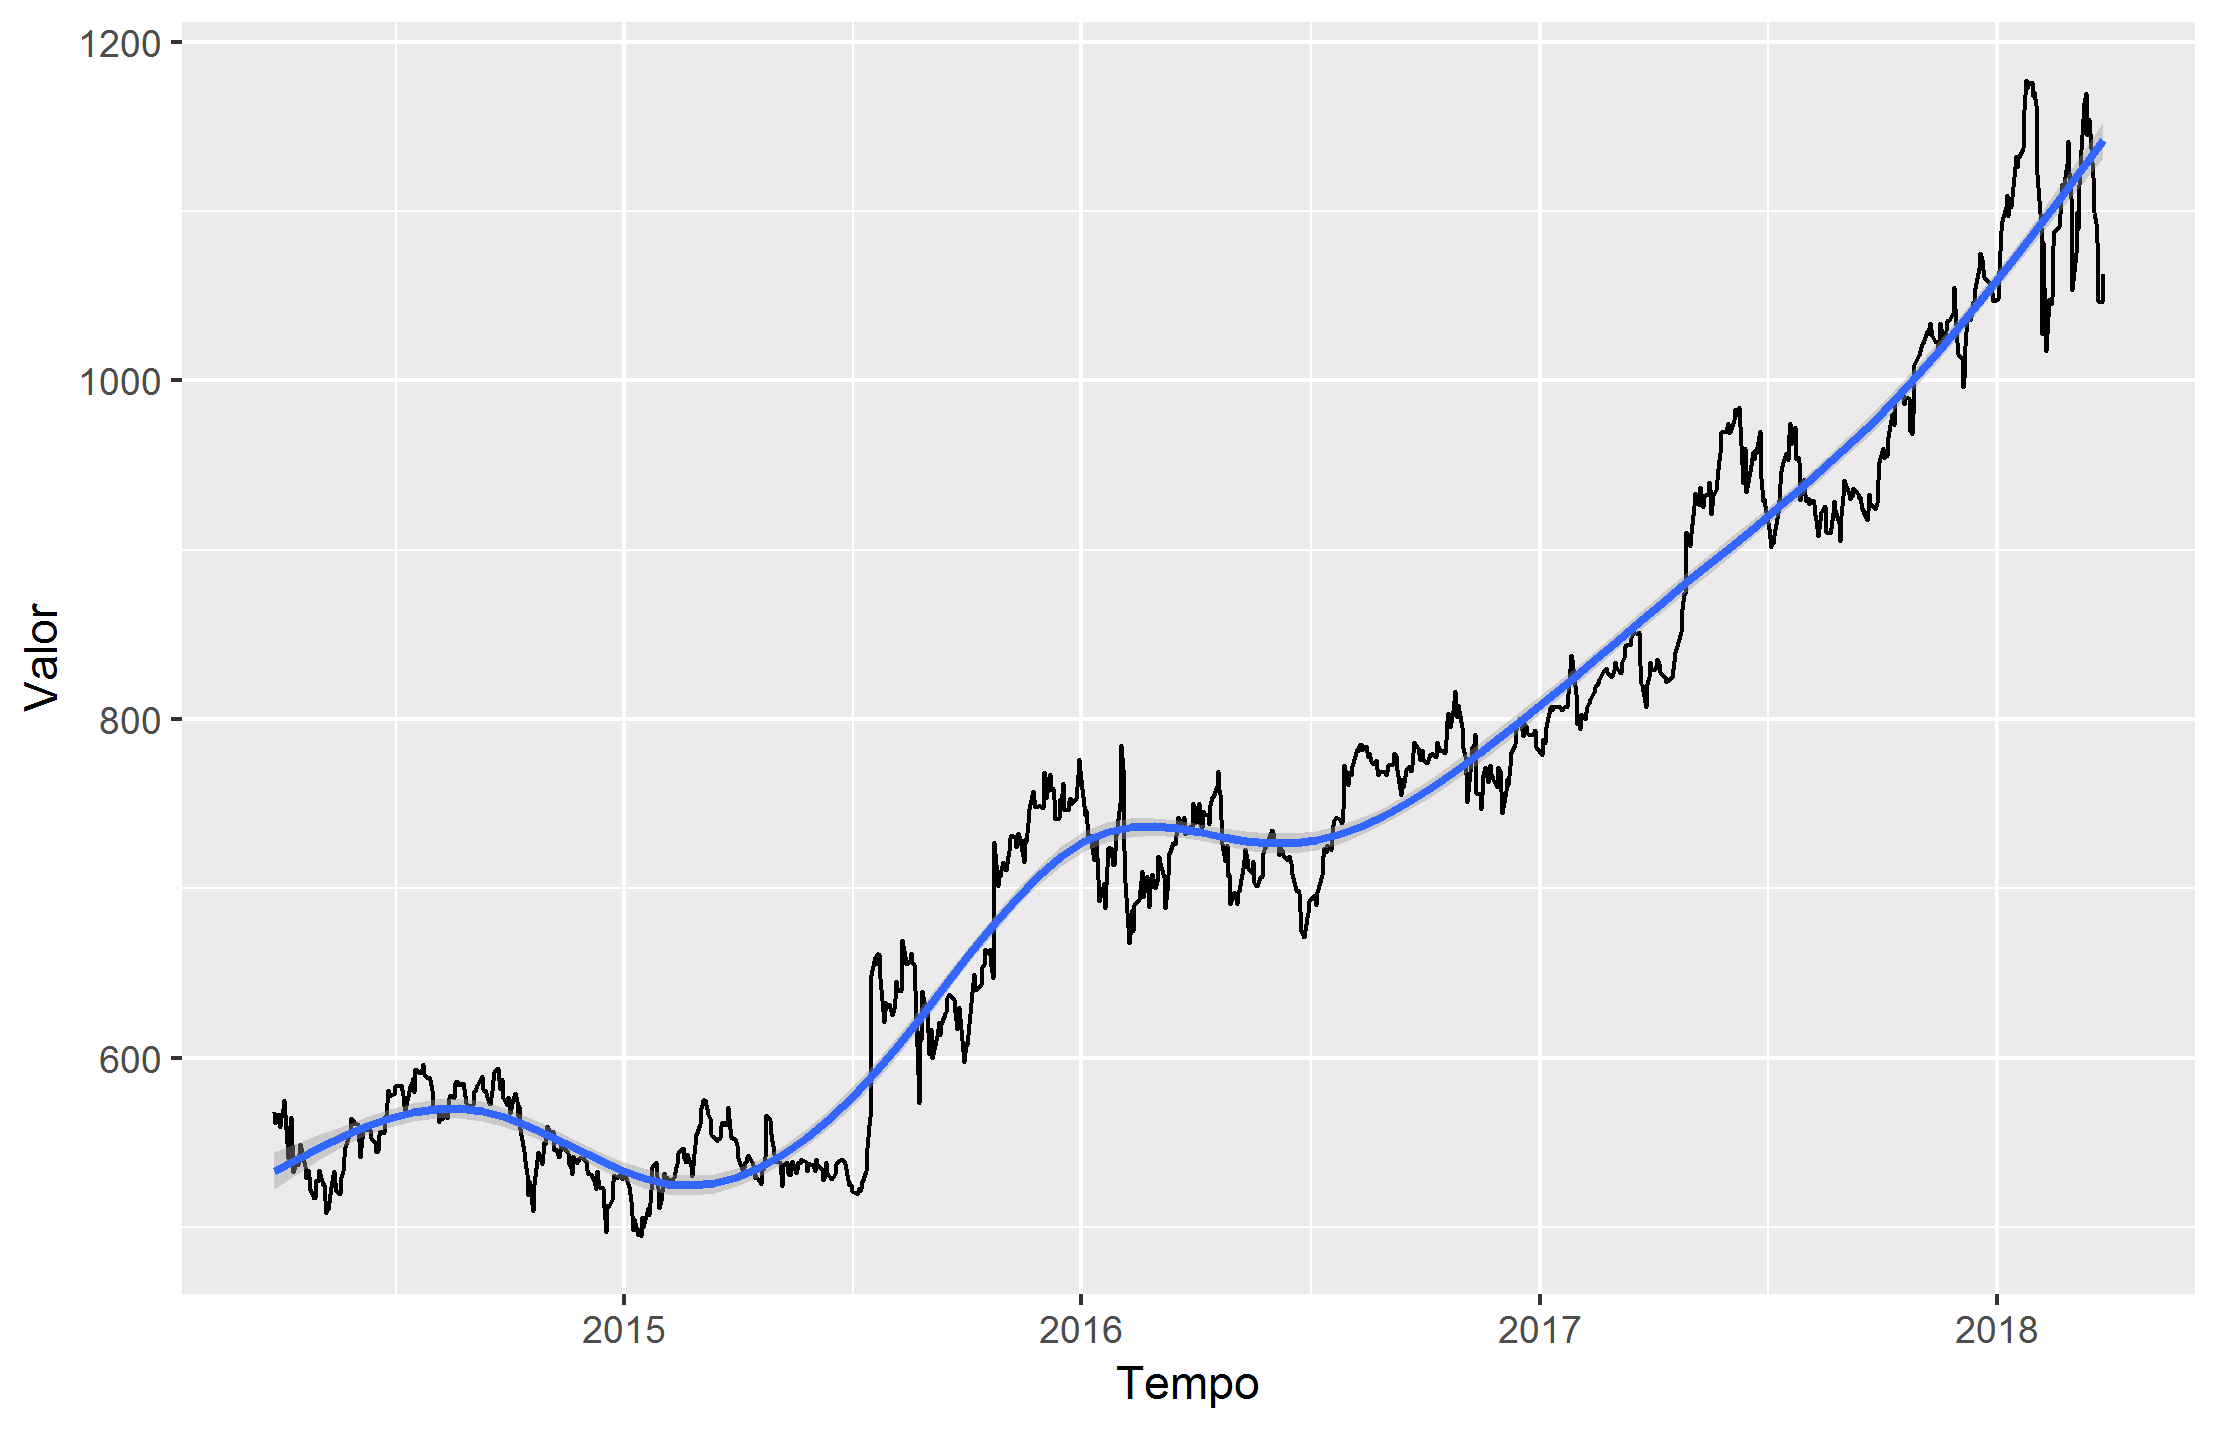
\includegraphics[scale=0.45]{stock}
	\caption{Valor de abertura das ações da Google na NASDAQ. Curva em preto: dados medidos. Curva em azul: curva ajustada aos dados medidos. Fonte: autoria própria, dados: Google Finance.}
\end{figure}}

\frame{\frametitle{Proposta do trabalho}

\begin{block}{Objetivo}
Estimar a produção de energia, a partir de dados de vento, em curtos intervalos de tempo por meio de um modelo que contemple o caráter estocástico, físico, real do vento.
\end{block}
	
}

\frame{\frametitle{Proposta do trabalho}

Para cumprir a proposta do trabalho é preciso:

\begin{itemize}
\item Fazer uma revisão da literatura
\item Entender fundamentos matemáticos: cálculo de Ito, teoria do caos, Monte Carlo
\item Entender os limites do estudo (precisão numérica, horizonte de previsão)
\item Simulação numérica
\item Entender como a estimativa de energia (de 20 anos) é feita
\item Comparação entre métodos e com dados medidos
\end{itemize}

}

\frame{\frametitle{Planejamento}\begin{figure}[h]
	\hspace*{-0.8cm}   
    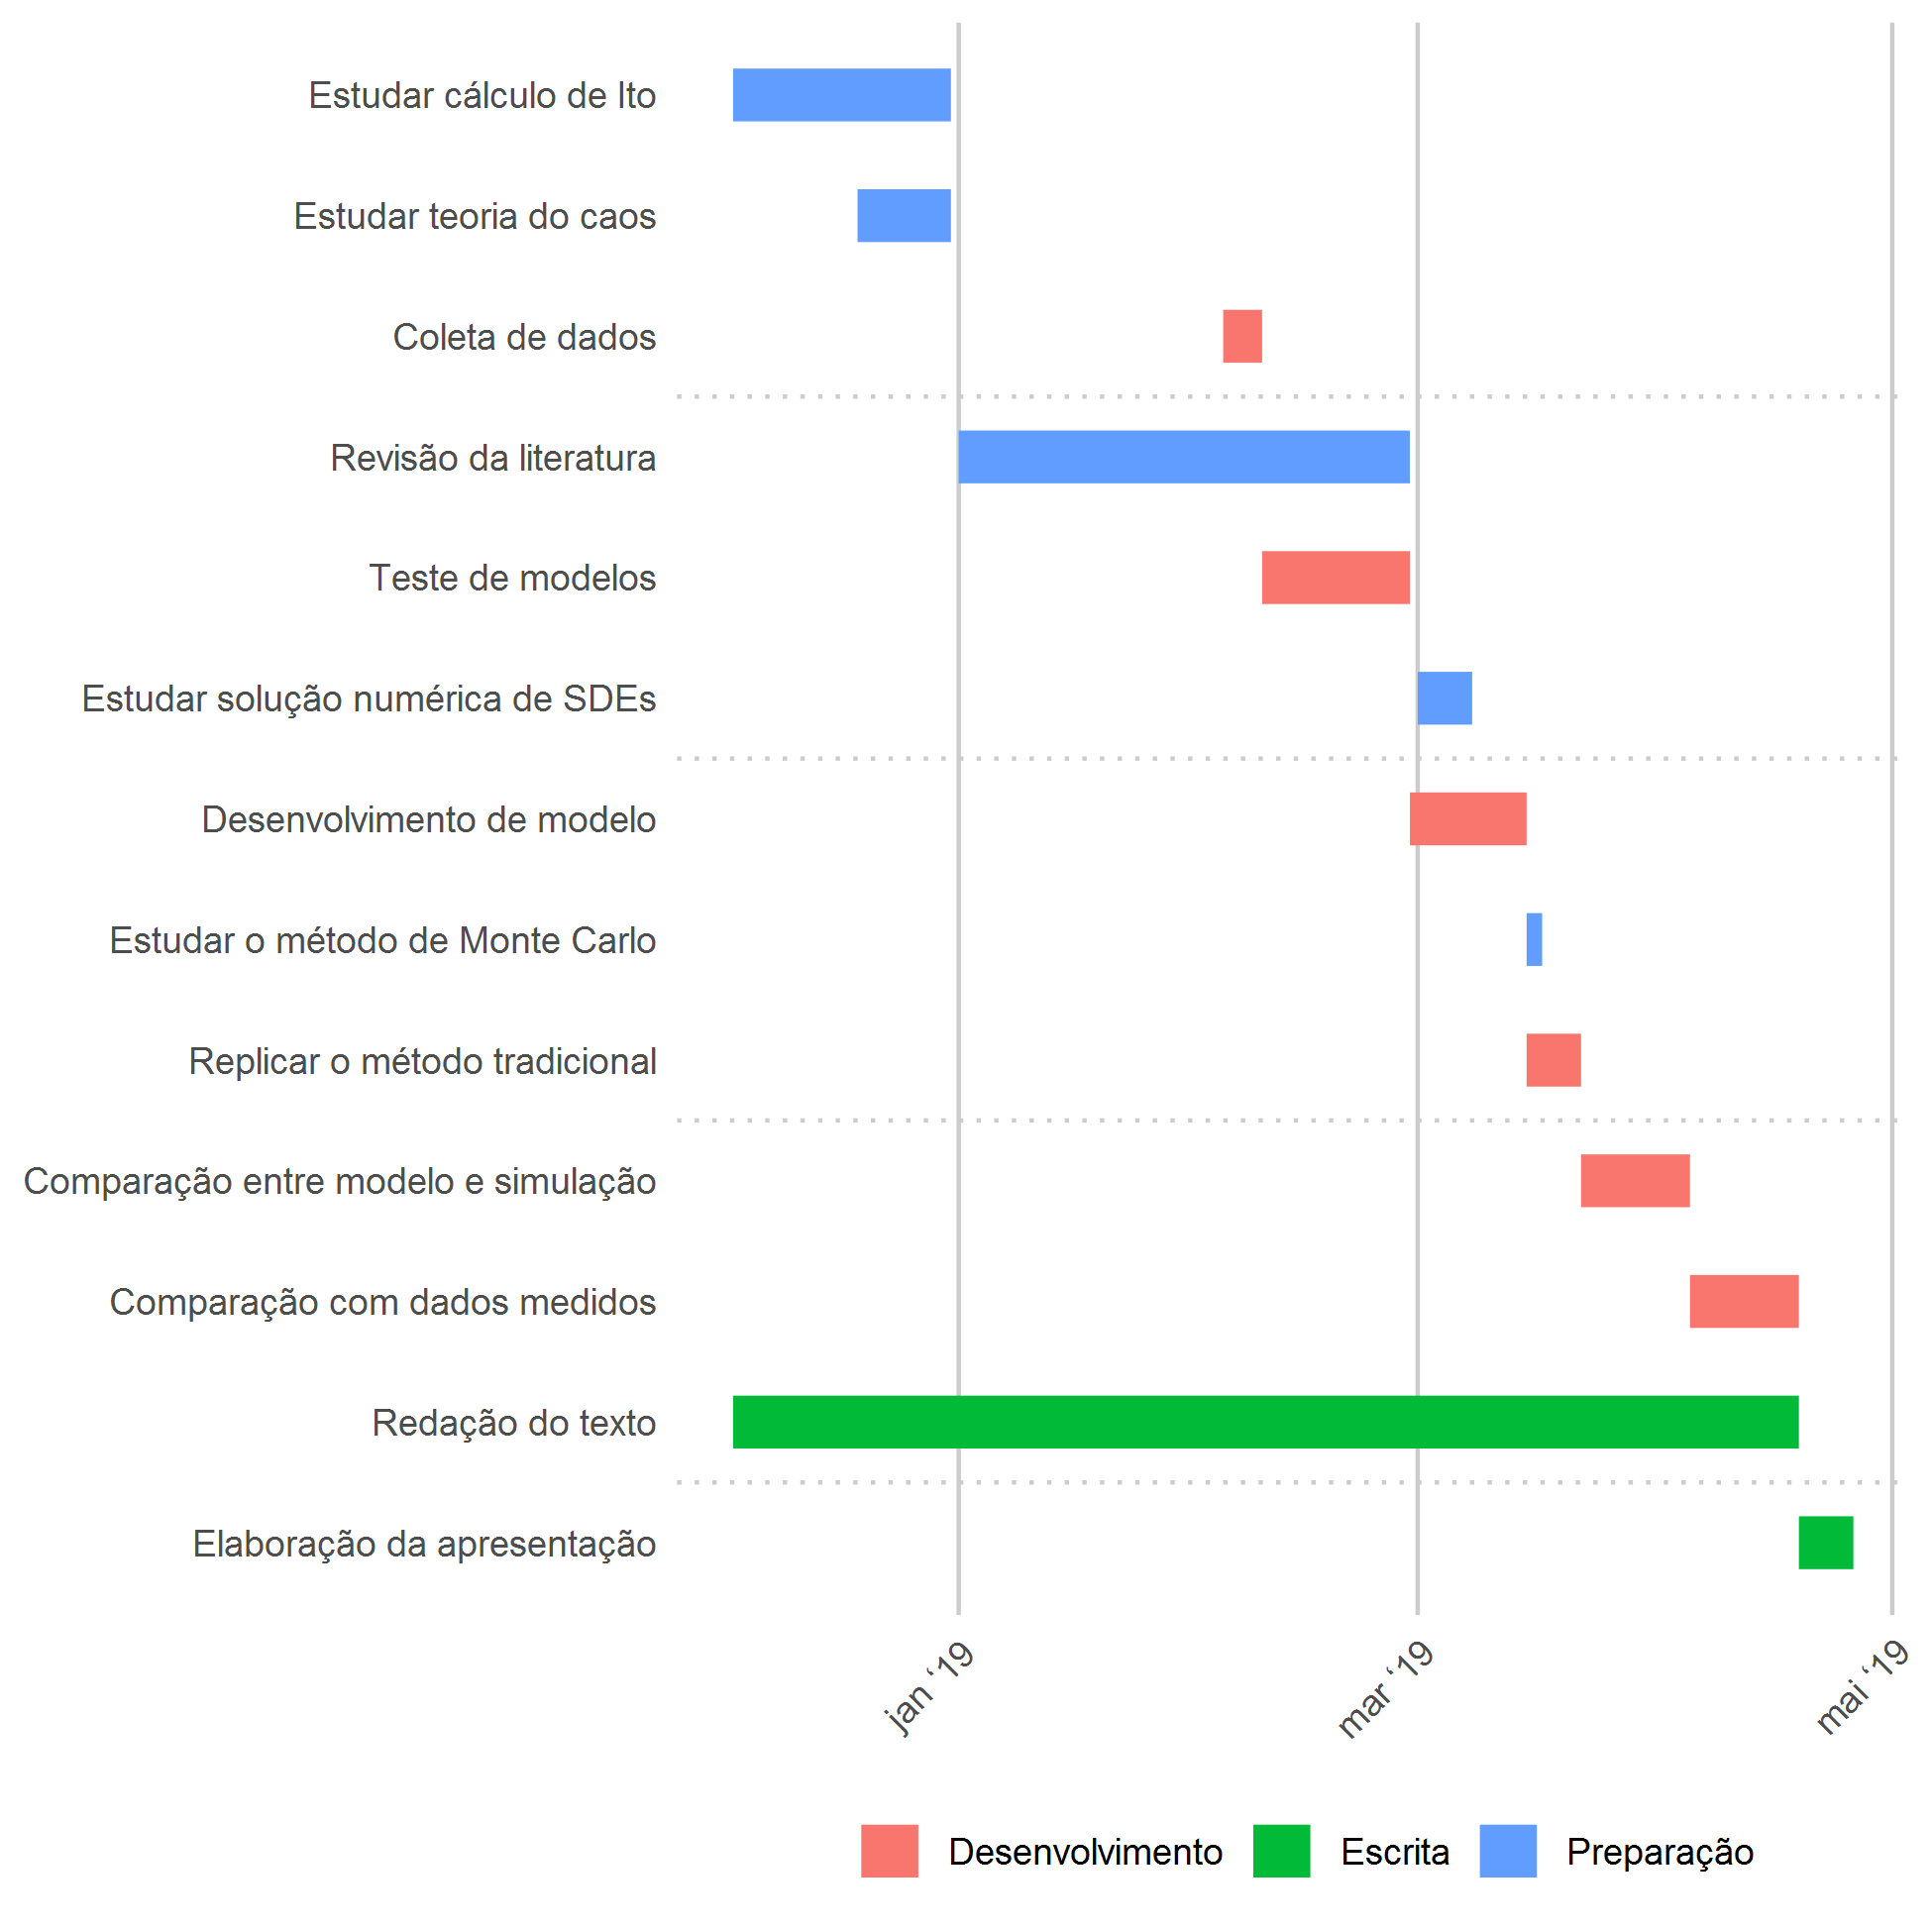
\includegraphics[scale=0.41]{gantt}
    \caption{Gráfico de Gantt do planejamento das etapas de desenvolvimento do presente trabalho. Fonte: autoria própria.}
    \centering
\end{figure}}

\end{document}
